\index{Linear time-invariant systems}{Linear time-invariant systems}
(LTI) are an important class of systems that can be analyzed easily in frequency domain. An LTI system is equivalent to \emph{\index{convolution}{convolution}} of the \emph{impulse response} of the system. 
The focus of this chapter is to learn more about what these concepts are. 

\section{Example: Running average filter}
Here's an example of a discrete-time system that you might use to smooth a noisy signal:
\begin{equation}
  y[n] = \frac{1}{15}\sum_{k=-7}^{7} x[n-k]\,\,.
  \label{eq:running_mean}
\end{equation}
What does this system do? It averages together 15 neighboring values of input signal $x[n]$. Figure \ref{fig:avg_filter} shows a demonstration of this system in action. 
The blue line indicates a noisy input signal $x[n]$, and the orange line depicts the output $y[n]$ of the running mean filter given in Equation \ref{eq:running_mean}. 
As you might expect, the output of the system is a smoother version of the input signal.
\begin{figure}
  \begin{center}
    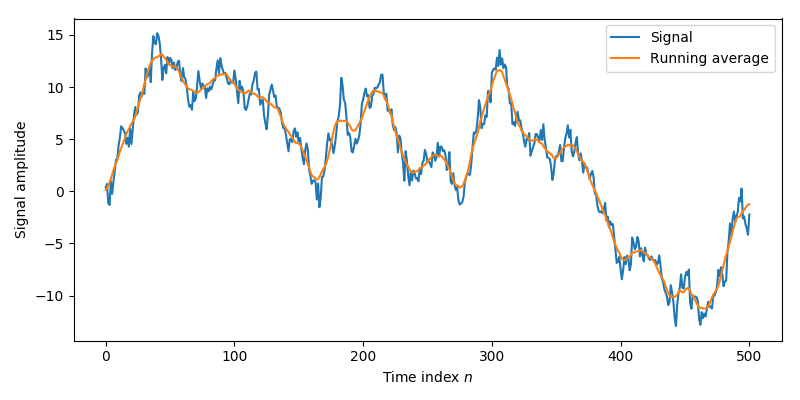
\includegraphics[width=\textwidth]{code/016_smoothing/smoothing.png}
  \end{center}
  \caption{A running average filter is often used to smooth a noisy
    signal. You can find the Python code used to produce this example
    in \texttt{016\_smoothing/smoothing.py}.}
  \label{fig:avg_filter}
\end{figure}

\section{Finite impulse response filter}
\begin{marginfigure}

\begin{center}
  \begin{tikzpicture}[node distance=3cm,auto,>=latex']
    \node [int] (a) {LTI};
    \node (b) [left of=a, coordinate] {a};
%    \node (c) [below=a,node distance=3cm] {a};

%\node [int, pin={[init]above:$p_0$}] (c) [right of=a] {$\frac{1}{s}$};
    \node [coordinate] (end) [right of=a]{};
    \path[->] (b) edge node {$x[n]$} (a);
    \path[->] (b) edge node [below]{$\delta[n]$} (a);

%\path[->] (a) edge node {$v$} (c);
    \draw[->] (a) edge node {$y[n]$} (end) ;
    \draw[->] (a) edge node [below]{$h[n]$} (end) ;

\end{tikzpicture}
\end{center}
\caption{Discrete-time LTI systems are characterized by an impulse response $h[n]$, which is the response of the LTI system to a unit impulse signal.}
\end{marginfigure}

The previous system shown in Equation \ref{eq:running_mean} is a special case of a more general type of discrete-time LTI system, 
known as a Finite Impulse Response (FIR) filter. This type of signal is often used in digital signal processing. 
An FIR filter is defined as follows:
\begin{equation}
  \boxed{
    y[n] = \sum_{k=-M}^{N} b_k x[n-k]\,\,.
  }
  \label{eq:fir_filter}
\end{equation}
The coefficients $b_k \in \mathbb{C}$ here are constant valued coefficients. As the name implies, there is a finite number of non-zero coefficients $b_k$. 
In the case of the running average filter in Equation \ref{eq:running_mean}, there would be 15 coefficients, which are all $b_k=1/15$.

\section{General discrete-time LTI system}
What if we allow there to be infinitely many coefficients for the system given in Equation \ref{eq:fir_filter}? We get the following:
\begin{equation}
    y[n] = \sum_{k=-\infty}^{\infty} b_k x[n-k] = \sum_{k=-\infty}^{\infty} b[k] x[n-k]\,\,.
\end{equation}
This turns out to be the general representation for arbitrary discrete-time LTI systems! In this case, it makes sense to think of the infinitely many coefficients $b_k$ as a signal $b[k]$.

For discrete-time LTI systems in general, the output of a system is given by a discrete-time convolution sum of the input signal $x[n]$ with an impulse response $h[n]$:

\begin{marginfigure}
  \begin{center}
          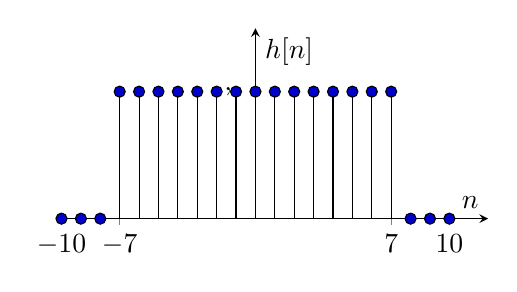
\begin{tikzpicture}
          \begin{axis}[width=7cm,height=4cm,ymin=0,xmin=-10,ymax=0.1,xmax=12,
         xtick={-10,-7,0,7,10},
              ytick={0,1,2,3},
              ytick={0,0.0667},
              yticklabel={,,},
          ylabel={$h[n]$},
      xlabel={$n$}, axis lines = center]
     \addplot+[ycomb,color=black] plot coordinates {(-10,0)(-9,0)(-8,0)(-7,0.0667)(-6,0.0667)(-5,0.0667)(-4,0.0667)(-3,0.0667)(-2,0.0667)(-1,0.0667)(0,0.0667)(1,0.0667)(2,0.0667)(3,0.0667)(4,0.0667)(5,0.0667)(6,0.0667)(7,0.0667)(8,0)(9,0)(10,0)};
  \end{axis}
  \end{tikzpicture}
  \end{center}
  \caption{The impulse response of the 15 point running mean filter described in Equation \ref{eq:running_mean}.}
\end{marginfigure}

\begin{equation}
  \boxed{
    y[n] = \mathcal{T}\{x[n]\}=\sum_{k=-\infty}^{\infty} h[k] x[n-k]\,\,.
  }
  \label{eq:conv_dlti}
\end{equation}
The impulse response is defined as follows:
\begin{equation}
  \boxed{
    h[n] = \mathcal{T}\{\delta[n]\}\,\,.
  \label{eq:conv_ireq}    
    }
\end{equation}
It is hopefully easy to see that Equation \ref{eq:conv_dlti} is valid for all LTI systems. %This was already briefly discussed earlier in the chapter on Fourier transforms.

A linear system $\mathcal{T}\{\cdot\}$\footnote{If linearity applies for two input signals $\mathcal{T}\{\alpha_1 s_1[n] + \alpha_2 s_2[n]\} = \alpha_1 \mathcal{T}\{s_1[n]\}+\alpha_2 \mathcal{T}\{s_2[n]\}$, it also applies for linear combinations of three or more signals.} must by definition satisfy the following relation:
\begin{equation}
  \mathcal{T}\left\{\sum_{k=-\infty}^{\infty} \alpha_k s_k[n]\right\} = \sum_{k=-\infty}^{\infty} \alpha_k \mathcal{T}\{s_k[n]\}\,\,.
  \label{eq:linearity_gen}
\end{equation}
Here $\alpha_k \in \mathbb{C}$ are arbitrary constants and $s_k[n]$ are arbitrary signals.

Time-invariance of $\mathcal{T}\{\cdot\}$, on the other hand, implies that for any time shift $k$ in the input, the output is correspondingly time shifted. 
This is valid for any input signal $x[n]$:
\begin{equation}
y[n-k] = \mathcal{T}\{x[n-k]\}\,\,,
\end{equation}
if 
\begin{equation}
y[n]=\mathcal{T}\{x[n]\}\,\,.
\end{equation}
It is possible to represent any signal $x[n]$ with the help of time-shifted unit impulse signals\sidenote{Recall that the discrete-time unit impulse is defined as: 
\begin{equation}
\delta[n] = \left\{
  \begin{array}{rcr}
    1 & \mathrm{when} & n=0 \\
    0 & \mathrm{otherwise} & \\
  \end{array}
\right.\,\,.
\end{equation}

It is the discrete-time equivalent of a Dirac delta function. The unit impulse is shown in Figure \ref{fig:dt_unit_impulse}.
}:
\begin{equation}
  x[n] = \sum_{k=-\infty}^{\infty} x[k]\delta[n-k]\,\,.
\end{equation}
Linearity implies that:
\begin{equation}
\mathcal{T}\{x[n]\} = \mathcal{T}\left\{\sum_{k=-\infty}^{\infty}x[k]\delta[n-k]\right\} = \sum_{k=-\infty}^{\infty}x[k] \mathcal{T}\{\delta[n-k]\}\,\,.
\end{equation}
\if 0
\begin{marginfigure}
\begin{center}
    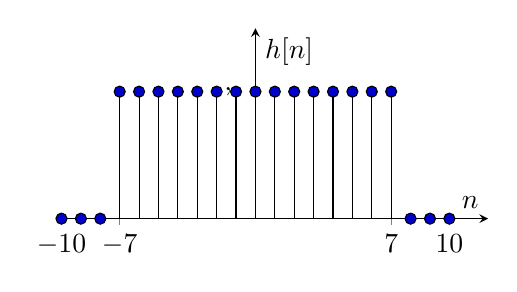
\begin{tikzpicture}
      \begin{axis}[width=7cm,height=4cm,ymin=0,xmin=-10,ymax=0.1,xmax=12,
                   xtick={-10,-7,0,7,10},
                  ytick={0,1,2,3},
             ytick={0,0.0667},
             yticklabel={,,},
             ylabel={$h[n]$},
             xlabel={$n$}, axis lines = center]
        \addplot+[ycomb,color=black] plot coordinates {(-10,0)(-9,0)(-8,0)(-7,0.0667)(-6,0.0667)(-5,0.0667)(-4,0.0667)(-3,0.0667)(-2,0.0667)(-1,0.0667)(0,0.0667)(1,0.0667)(2,0.0667)(3,0.0667)(4,0.0667)(5,0.0667)(6,0.0667)(7,0.0667)(8,0)(9,0)(10,0)};
      \end{axis}
     \end{tikzpicture}
\end{center}
\caption{The impulse response of the 15 point running mean filter described in Equation \ref{eq:running_mean}.}
\end{marginfigure}
\fi
\noindent The equation above is the same as Equation \ref{eq:linearity_gen} with $s_k[n] = \delta[n-k]$ and $\alpha_k=x[k]$.  Due to time-invariance,
we can relate the impulse response $h[n]$ delayed by $k$ to the term
on the right-hand side above. If a unit impulse fed into the system is
\begin{equation}
h[n] = \mathcal{T}\{\delta[n]\},
\end{equation}
\begin{marginfigure}
  \begin{center}
    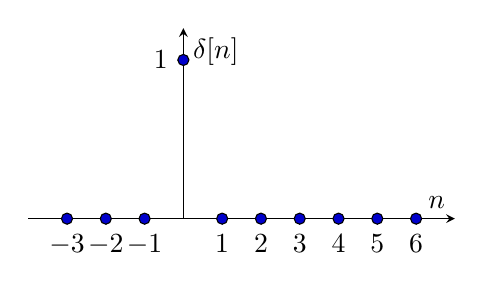
\begin{tikzpicture}
      \begin{axis}[width=7cm,height=4cm,ymin=0,xmin=-4,ymax=1.2,xmax=7,
                   xtick={-3,-2,-1,0,1,2,3,4,5,6},
                   ytick={0,1,2,3},
                   ylabel={$\delta[n]$},
                   xlabel={$n$}, axis lines = center]
          \addplot+[ycomb,color=black] plot coordinates {(-3,0) (-2,0) (-1,0) (0,1) (1,0) (2,0) (3,0) (4,0) (5,0) (6,0)};
      \end{axis}
     \end{tikzpicture}
     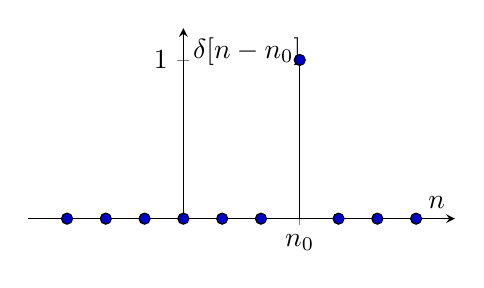
\begin{tikzpicture}
        \begin{axis}[width=7cm,height=4cm,ymin=0,xmin=-4,ymax=1.2,xmax=7,
          xtick={3},
          xticklabels={$n_0$},
          ytick={0,1,2,3},
          ylabel={$\delta[n-n_0]$},
          xlabel={$n$}, axis lines = center]
          \addplot+[ycomb,color=black] plot coordinates {(-3,0) (-2,0) (-1,0) (0,0) (1,0) (2,0) (3,1) (4,0) (5,0) (6,0)};
        \end{axis}
      \end{tikzpicture}
  \end{center}
  \caption{Discrete-time unit impulse signal $\delta[n]$ and a time-shifted version $\delta[n-n_0]$ centered at $n=n_0$.}
  \label{fig:dt_unit_impulse}
\end{marginfigure}
then a time-shifted unit impulse corresponds to a time-shifted output:
\begin{equation}
h[n-k] = \mathcal{T}\{\delta[n-k]\}\,\,.
\end{equation}
Therefore, the output of an LTI system for an arbitrary input signal
$x[n]$ can be expressed using the impulse response $h[n]$ as follows:
\begin{equation}
  y[n] = \sum_{k=-\infty}^{\infty} x[k]h[n-k].
  \label{eq:convolution_intro}
\end{equation}
This type of equation is known as a discrete-time convolution sum. We have now shown that any discrete-time LTI system can be represented with such a convolution sum. 
Note that Equation \ref{eq:convolution_intro} isn't quite yet the same as Equation \ref{eq:conv_dlti}. We will later show that the convolution sum is commutative, i.e., that:
\begin{equation}
 \sum_{k=-\infty}^{\infty} x[k]h[n-k] = \sum_{k=-\infty}^{\infty} h[k]x[n-k].
\end{equation}
Which completes the proof.

\subsection{Example: Impulse response of an FIR filter}
An FIR filter (Equation \ref{eq:fir_filter}) has the following impulse response:
\begin{equation}
h[n] = \sum_{k=-M}^{N} b_k \delta[n-k]\,\,.
\end{equation}
The signal $h[n]$ contains the values of the filter coefficients $h[n]=b_n$. Since there are a finite number of coefficients $b_k$, the impulse response $h[n]$ 
has non-zero values only in a finite range of samples. This is also where the name ``finite impulse response'' comes from.
\begin{marginfigure}
\begin{center}
  \begin{tikzpicture}[node distance=2cm,auto,>=latex']
    \node [int] (a) {FIR filter ($b_k$)};
    \node (b) [left of=a, coordinate] {a};
%    \node (c) [below=a,node distance=3cm] {a};

%\node [int, pin={[init]above:$p_0$}] (c) [right of=a] {$\frac{1}{s}$};
    \node [coordinate] (end) [right of=a]{};
    \path[->] (b) edge node {$\delta[n]$} (a);
    %\path[->] (a) edge node {$v$} (c);
    \draw[->] (a) edge node {$h[n]$} (end) ;
\end{tikzpicture}
\end{center}
\caption{The impulse response of an FIR filter is a signal that contains the coefficients. For a finite number of coefficients $b_k$, the length of 
the non-zero portion of the impulse response is finite, and hence the name FIR.}
\end{marginfigure}


\section{Impulse response}
Linear time-invariant (LTI) systems are fully characterized by an \index{impulse response} impulse response $h(t)$. 
This impulse response is obtained by feeding a unit impulse into the LTI system:
\begin{equation}
\boxed{
h(t) = \mathcal{T}\{\delta(t)\}\,\,.
}
\end{equation}
Using an impulse response, it is possible to represent the output of any LTI system as a convolution between the impulse response and the input signal.
\begin{equation}
\boxed{
y(t) = \mathcal{T}\{x(t)\} = h(t)*x(t) = \int_{-\infty}^{\infty} h(\tau)x(t-\tau)d\tau\,\,.
}
\end{equation}
Let's prove this. We'll first need to represent an arbitrary signal as a sum of unit impulses:
\begin{equation}
x(t)  = \int_{-\infty}^{\infty} x(\tau) \delta(t-\tau) d\tau\,\,.
\end{equation}
One way to think of this integral is that the unit impulse $\delta(t-\tau)$ ``selects'' the value of $x(\tau)$ where $\tau=t$. 
Another way to think of this is that the Dirac delta functions form a set of basis functions for representing the signal $x(t)$.

\tikzstyle{int}=[draw, minimum size=2em]
\tikzstyle{init} = [pin edge={to-,thin,black}]

\begin{marginfigure}
\begin{center}

  \begin{tikzpicture}[node distance=3cm,auto,>=latex']

    \node [int] (a) [align=center]{LTI };
    \node (b) [left of=a, coordinate] {a};
%    \node (c) [below=a,node distance=3cm] {a};

%\node [int, pin={[init]above:$p_0$}] (c) [right of=a] {$\frac{1}{s}$};
    \node [coordinate] (end) [right of=a]{};
    \path[->] (b) edge node {$\delta(t)$} (a);
  %  \path[->] (b) edge node [below]{$\delta(t)$} (a);

%\path[->] (a) edge node {$v$} (c);
    \draw[->] (a) edge node {$h(t)$} (end) ;
 %   \draw[->] (a) edge node [below]{$h(t)$} (end) ;

\end{tikzpicture}

\end{center}
\caption{A linear time-invariant system is characterized by an impulse response.}
\end{marginfigure}

You may recall that linearity of the system $\mathcal{T}\{\cdot\}$ implies that:
\begin{equation}
\mathcal{T}\{c_1 \delta(t-\tau_1) + c_2 \delta(t-\tau_2)\} = c_1 \mathcal{T}\{\delta(t-\tau_1)\}+ c_2 \mathcal{T}\{\delta(t-\tau_2)\}\,\,.
\end{equation}
Here I've used $\delta(t-\tau_1)$ and $\delta(t-\tau_2)$ as two different input signals. The terms $c_1,c_2\in \mathbb{C}$ are arbitrary complex valued constants.

Linearity must therefore also apply for the linear combination of an arbitrary number of inputs:
\begin{equation}
\mathcal{T}\left\{\sum_n x_n \delta(t-\tau_n)\right\} = \sum_n x_n \mathcal{T}\{\delta(t-\tau_n)\}\,\,.
\end{equation}
Linearity can be extended even further into a continuous linear combination:
\begin{equation}
\mathcal{T}\left\{\int_{-\infty}^{\infty} x(\tau)\delta(t-\tau)d\tau\right\} = \int_{-\infty}^{\infty} x(\tau) \mathcal{T}\{\delta(t-\tau)\} d\tau\,\,.
\end{equation}
We can simplify the right-hand side and get:
\begin{equation}
\int_{-\infty}^{\infty} x(\tau) \mathcal{T}\{\delta(t-\tau)\} d\tau = \mathcal{T}\left\{x(t)\right\}\,\,.
\end{equation}
In order to simplify the left-hand side, we have to rely on the property of \emph{time-invariance}. That is:
\begin{equation}
h(t) = \mathcal{T}\{\delta(t)\} \Rightarrow h(t-\tau) = \mathcal{T}\{\delta(t-\tau)\}\,\,.
\end{equation}
This now completes our proof:
\begin{equation}
y(t)=\int_{-\infty}^{\infty} x(\tau) h(t-\tau) d\tau = \mathcal{T}\left\{x(t)\right\}\qed\,\,.
\end{equation}
The output of a linear time-invariant system $y(t)=\mathcal{T}\{x(t)\}$ is a convolution of the system's 
impulse response $h(t)=\mathcal{T}\{\delta(t)\}$ with the input signal $x(t)$ fed into the system.

\section{Convolution}

A convolution operation is defined for both continuous-time and
discrete-time signals. As we just saw, a convolution operation can be
interpreted as an LTI system applied to a signal.

The continuous-time convolution is defined as an integral:
\begin{equation}
\boxed{
  a(t)*b(t) = \int_{-\infty}^{\infty}a(\tau)b(t-\tau)d\tau\,\,.
}
\end{equation}
The discrete-time convolution is defined as a sum:
\begin{equation}
\boxed{
  a[n]*b[n] = \sum_{k=-\infty}^{\infty}a[k]b[n-k]\,\,.
}
\end{equation}

\section{Properties of a convolution}
The properties of the convolution operation are shown in Table \ref{con:table}. The same properties also exist for the continuous-time convolution
operation. 
\begin{table}
    \centering
    \caption{Table of convolution properties}
    \label{con:table}
    \begin{tabular}{|c|c|}
    \hline
    Property     & Equation \\ \hline
    identity     & $x[n]*\delta[n]=x[n]$ \\ \hline
    commutative  & $a[n] * b[n] = b[n] * a[n]$ \\ \hline
    associative  & $(a[n]*b[n]) * c[n] = a[n] * ( b[n] * c[n])$ \\ \hline
    distributive & $a[n]*(b[n]+c[n]) = a[n]*b[n] + a[n]*c[n]$ \\ \hline
    \end{tabular}
\end{table}

The proof of the identity property is clear, and the commutative property is left as an exercise. The associative property takes a bit more work, and the proof is as follows: 
\begin{proof}
Using the definition of the convolution operation twice:
\begin{align}
(a[n]*b[n])*c[n] &= \sum_{k}\underbrace{\left(\sum_\ell a[\ell]b[k-\ell]\right)}_{a[k]*b[k]} c[n-k] \\
                 &= \sum_{k}\sum_\ell a[\ell]b[k-\ell]c[n-k]
\end{align}
For the other ordering:
\begin{align}
a[n]*(b[n]*c[n]) &= \sum_{\ell} a[\ell] \Big(\underbrace{\sum_m b[m]c[(n-m)}_{b[n]*c[n]}-\ell]\Big)\\
                 &= \sum_{\ell} \sum_m a[\ell] b[m]c[(n-m)-\ell]\,\,.
\end{align}
If we now substitute: $m=k-\ell$, then $n-m-\ell=n-k$, which gives
\begin{align}
a[n]*(b[n]*c[n]) &= \sum_{k} \underbrace{\left(\sum_{\ell} a[\ell] b[k-\ell]\right)}_{a[k]*b[k]} c[n-k]\,\,,
\end{align}
which is the same as $(a[n]*b[n])*c[n]$, which completes the proof.
\end{proof}

\begin{marginfigure}
\begin{center}
  \begin{tikzpicture}[node distance=3cm,auto,>=latex']

    \node [int] (a) {LTI $(h_1[n])$};
    \node [above of=a, node distance=1cm] (in) {$x[n]$};
    \node [int, below of=a, node distance=1cm] (b) {LTI $(h_2[n])$};
    \node [below of=b, node distance=1cm] (out) {$y[n]$};
    \path[->] (a) -> (b);
    \draw[->] (a) -> (b);
    \path[->] (in) -> (a);
    \draw[->] (in) -> (a);
    \path[->] (b) -> (out);
    \draw[->] (b) -> (out);
    
    \node [int, right of=a,node distance=2cm] (a3) {LTI $(h_3[n])$};
    \node [above of=a3, node distance=1cm] (in3) {$x[n]$};
    \node [below of=a3, node distance=1cm] (out3) {$y[n]$};
    \path[->] (in3) -> (a3);
    \draw[->] (in3) -> (a3);
    \path[->] (a3) -> (out3);
    \draw[->] (a3) -> (out3);
    
\end{tikzpicture}
\end{center}
\caption{A consequence of the associative property of convolution is
  that two LTI systems characterized with $h_1[n]$ and $h_2[n]$ can be
  combined as a single LTI system with impulse response
  $h_3[n]=h_1[n]*h_2[n]$.}
\label{fig:cascade_lti1}
\end{marginfigure}

A consequence of the associative property is that if we have two LTI
systems that are applied to an input signal $x[n]$ in series, we can
come up with a single LTI system that is equivalent to two \index{chained 
LTI system} chained LTI systems:
\begin{equation}
  y[n] = (x[n]*h_1[n])*h_2[n] = x[n]*h_3[n]\,\,.
\end{equation}
Here $h_3[n]=h_1[n]*h_2[n]$. This is depicted in Figure
\ref{fig:cascade_lti1}. This property can be extended to an arbitrary
number of systems that are connected together in series.

\subsection{Distributive}

\begin{marginfigure}

\begin{center}
  \begin{tikzpicture}[node distance=3cm,auto,>=latex']

    \node [draw,shape=circle](p) {$+$};
    \node [int, above left of=p,node distance=1.5cm] (a1) {LTI $(h[n])$};
    \node [int, above right of=p,node distance=1.5cm] (a2) {LTI $(h[n])$};
    \node [above of=a1,node distance=1cm] (i1) {$x_1[n]$};
    \node [above of=a2,node distance=1cm] (i2) {$x_2[n]$};
    \node [below of=p,node distance=1cm] (o1) {$y[n]$};

    \path[->] (i1) -> (a1);
    \draw[->] (i1) -> (a1);
    \path[->] (i2) -> (a2);
    \draw[->] (i2) -> (a2);
    
    \path[->] (a1) -> (p);
    \draw[->] (a1) -> (p);
    \path[->] (a2) -> (p);
    \draw[->] (a2) -> (p);
    \path[->] (p) -> (o1);
    \draw[->] (p) -> (o1);
    
    
    \node [int, right of=a2,node distance=2cm] (a3) {LTI $(h[n])$};
    \node [above of=a3, node distance=1cm] (in3) {$x_1[n]+x_2[n]$};
    \node [below of=a3, node distance=1cm] (out3) {$y[n]$};
    \path[->] (in3) -> (a3);
    \draw[->] (in3) -> (a3);
    \path[->] (a3) -> (out3);
    \draw[->] (a3) -> (out3);
    
\end{tikzpicture}
\end{center}
\caption{A consequence of the distributive property is linearity.}
\label{fig:sum_lti}
\end{marginfigure}

The convolution is distributive:
\begin{equation}
a[n]*(b[n]+c[n]) = a[n]*b[n] + a[n]*c[n]\,\,.
\end{equation}

\begin{proof}
\begin{align}
a[n]*(b[n]+c[n]) & = \sum_{k=-\infty}^{\infty} a[k](b[n-k]+c[n-k]) \\
 & = \sum_{k=-\infty}^{\infty} a[k]b[n-k]+ \sum_{k=-\infty}^{\infty} a[k]c[n-k]\,\,.
\end{align}
\end{proof}

An example application of this property is shown in Figure
\ref{fig:sum_lti}. Signals $x_1[n]$ and $x_2[n]$ fed into an identical
LTI systems separately and then added together is equivalent to the
sum of the signals fed into a single LTI system.


\section{Example: Convolution animations}

Animations of the convolution operation for various example systems
can be found here: \url{http://kaira.uit.no/juha/fir_animation/}. The
code for creating such animations can be obtained from GitHub:
\url{https://github.com/jvierine/signal_processing/tree/master/017_fir_animation}.



